\documentclass{article}


% if you need to pass options to natbib, use, e.g.:
%     \PassOptionsToPackage{numbers, compress}{natbib}
% before loading neurips_2024


% ready for submission
\usepackage{neurips_2024}


% to compile a preprint version, e.g., for submission to arXiv, add add the
% [preprint] option:
%     \usepackage[preprint]{neurips_2024}


% to compile a camera-ready version, add the [final] option, e.g.:
%     \usepackage[final]{neurips_2024}


% to avoid loading the natbib package, add option nonatbib:
%    \usepackage[nonatbib]{neurips_2024}


\usepackage[utf8]{inputenc} % allow utf-8 input
\usepackage[T1]{fontenc}    % use 8-bit T1 fonts
\usepackage{hyperref}       % hyperlinks
\usepackage{url}            % simple URL typesetting
\usepackage{booktabs}       % professional-quality tables
\usepackage{amsfonts}       % blackboard math symbols
\usepackage{nicefrac}       % compact symbols for 1/2, etc.
\usepackage{microtype}      % microtypography
\usepackage{xcolor}         % colors
\usepackage{graphicx}


\title{Formatting Instructions For NeurIPS 2024}


% The \author macro works with any number of authors. There are two commands
% used to separate the names and addresses of multiple authors: \And and \AND.
%
% Using \And between authors leaves it to LaTeX to determine where to break the
% lines. Using \AND forces a line break at that point. So, if LaTeX puts 3 of 4
% authors names on the first line, and the last on the second line, try using
% \AND instead of \And before the third author name.


\author{%
  Nguyen Ngo Viet Trung \thanks{Use footnote for providing further information
    about author (webpage, alternative address)---\emph{not} for acknowledging
    funding agencies.} \\
  Department of Computer Science\\
  Cranberry-Lemon University\\
  Pittsburgh, PA 15213 \\
  \texttt{hippo@cs.cranberry-lemon.edu} \\
  % examples of more authors
  % \And
  % Coauthor \\
  % Affiliation \\
  % Address \\
  % \texttt{email} \\
  % \AND
  % Coauthor \\
  % Affiliation \\
  % Address \\
  % \texttt{email} \\
  % \And
  % Coauthor \\
  % Affiliation \\
  % Address \\
  % \texttt{email} \\
  % \And
  % Coauthor \\
  % Affiliation \\
  % Address \\
  % \texttt{email} \\
}

\author{%
  Nguyen Ngo Viet Trung \\
  Institute of Artificial Intelligence\\
  University of Engineering and Technology - VNU-UET\\
  Ha Noi, Viet Nam \\
  22022598@vnu.edu.vn \\
  }



  

\begin{document}


\maketitle


\begin{abstract}
  This is abstract
\end{abstract}


\section{Introduction}

Reasoning is an essential aspect of artificial intelligence, with applications 
spanning various domains such as problem-solving, theorem proving, 
decision-making, and robotics (Manning, 2022). According to the book Thinking, 
Fast and Slow (Daniel, 2017), humans possess two cognitive systems: "System 1" 
and "System 2." "System 1" operates quickly, relying on instincts, emotions, 
intuition, and unconscious processes. In contrast, "System 2" functions more 
slowly, handling tasks that require reasoning, such as algorithmic reasoning, 
logical analysis, and mathematical abilities. Reasoning plays a crucial role 
as one of the key functions of "System 2" (Bengio, 2017; Weston and Sukhbaatar, 
2023). 

Reasoning can be divided into two main types: formal language reasoning and 
natural language reasoning g (Reiter, 1975; Berzonsky, 1978; Teig and Scherer, 
2016; Yu et al., 2023a; Zhao et al., 2023b; Li et al., 2023u). Formal language 
reasoning is commonly used in fields such as formal verification of software and hardware 
systems, theorem proving, and automated reasoning (Reiter, 1975; Berzonsky, 1978). 
On the other hand, natural language reasoning enables more intuitive human-computer 
interactions and supports tasks such as question answering (Shao et al., 2023;
Jiang et al., 2021c), information retrieval l (Zhu et al., 2023d; Ai et al., 2023), text 
summarizationn (Liu et al., 2023n), and sentiment analysis (Yu et al., 2023a; Araci, 2019;
Barbieri et al., 2021).

Since their inception, foundation models (Bommasani et al., 2021)  have demonstrated 
remarkable effectiveness in various fields such as natural language processing 
(Qiao et al., 2022), computer vision (Wang et al., 2023h), and multimodal tasks  
(Li, 2023). Foundation models typically consist of billions of parameters and 
undergo(pre-)training using self-supervised learning (Jain et al., 2023) on a 
broad dataset (Bommasani et al., 2021). . After (pre-)trained, foundation models 
can be fine-tuned to tackle a wide range of tasks through methods such as task-specific 
fine-tuning, linear probing, or prompt engineering, demonstrating remarkable 
generalizability and impressive accuracy (Bommasani et al., 2021; Qiu et al., 2023a)

As a rapidly growing field in artificial intelligence research, reasoning with 
foundation models aims to develop models capable of understanding and interacting 
with complex information in a more human-like manner. These models are designed to 
reason about abstract concepts and make decisions based on logical rules. First, 
reasoning with foundation models enables the application of prior knowledge and 
domain expertise. Logical rules can be derived from expert knowledge or formalized 
from existing ontologies or knowledge graphs. By leveraging prior knowledge, these 
models can benefit from a better understanding of the problem domain and make more 
informed decisions. Second, reasoning with foundation models can enhance robustness 
and generalization capabilities. By incorporating the information contained in large 
datasets, these models are better equipped to handle situations involving limited data 
or scenarios not encountered during deployment. This enables the creation of more 
reliable and robust models suitable for real-world applications.

Reasoning encompasses a wide range of aspects, including Commonsense Reasoning, 
Mathematical Reasoning, Logical Reasoning, Causal Reasoning, Visual Reasoning, 
Audio Reasoning, Multimodal Reasoning, Embodied Reasoning, and Defeasible Reasoning. 
In this study, we focus on two specific aspects of reasoning: Commonsense Reasoning 
and Causal Reasoning.



% \subsection{Style}


% Papers to be submitted to NeurIPS 2024 must be prepared according to the
% instructions presented here. Papers may only be up to {\bf nine} pages long,
% including figures. Additional pages \emph{containing only acknowledgments and
% references} are allowed. Papers that exceed the page limit will not be
% reviewed, or in any other way considered for presentation at the conference.


% The margins in 2024 are the same as those in previous years.


% Authors are required to use the NeurIPS \LaTeX{} style files obtainable at the
% NeurIPS website as indicated below. Please make sure you use the current files
% and not previous versions. Tweaking the style files may be grounds for
% rejection.


% \subsection{Retrieval of style files}`'


% The style files for NeurIPS and other conference information are available on
% the website at
% \begin{center}
%   \url{http://www.neurips.cc/}
% \end{center}
% The file \verb+neurips_2024.pdf+ contains these instructions and illustrates the
% various formatting requirements your NeurIPS paper must satisfy.


% The only supported style file for NeurIPS 2024 is \verb+neurips_2024.sty+,
% rewritten for \LaTeXe{}.  \textbf{Previous style files for \LaTeX{} 2.09,
%   Microsoft Word, and RTF are no longer supported!}


% The \LaTeX{} style file contains three optional arguments: \verb+final+, which
% creates a camera-ready copy, \verb+preprint+, which creates a preprint for
% submission to, e.g., arXiv, and \verb+nonatbib+, which will not load the
% \verb+natbib+ package for you in case of package clash.


% \paragraph{Preprint option}
% If you wish to post a preprint of your work online, e.g., on arXiv, using the
% NeurIPS style, please use the \verb+preprint+ option. This will create a
% nonanonymized version of your work with the text ``Preprint. Work in progress.''
% in the footer. This version may be distributed as you see fit, as long as you do not say which conference it was submitted to. Please \textbf{do
%   not} use the \verb+final+ option, which should \textbf{only} be used for
% papers accepted to NeurIPS.


% At submission time, please omit the \verb+final+ and \verb+preprint+
% options. This will anonymize your submission and add line numbers to aid
% review. Please do \emph{not} refer to these line numbers in your paper as they
% will be removed during generation of camera-ready copies.


% The file \verb+neurips_2024.tex+ may be used as a ``shell'' for writing your
% paper. All you have to do is replace the author, title, abstract, and text of
% the paper with your own.


% The formatting instructions contained in these style files are summarized in
% Sections \ref{gen_inst}, \ref{headings}, and \ref{others} below.




\section{Background}
\subsection{Difinition of Reasoning}

Reasoning is a broad and multifaceted concept that manifests in various contexts. 
It encompasses cognitive and logical processes used to analyze information, draw 
inferences, reach conclusions, and construct coherent arguments. Reasoning can be 
observed across numerous domains such as scientific research, problem-solving, and 
decision-making. The purpose of reasoning is to enable individuals to connect pieces 
of information, evaluate relationships, and make informed judgments or solutions. 

Beyond its broad definition, the term “reasoning” also carries specific meanings across various fields:
\begin{itemize}
    \item In Philosophy (Cognitive Reasoning): Refers to modeling the human ability to draw meaningful conclusions even with incomplete and inconsistent knowledge. This includes ensuring that all processes, from acquiring and updating knowledge to drawing conclusions, are deployable and executable on appropriate hardware.
    \item In Logic (Logical Reasoning): Involves a systematic thought process where conclusions are derived methodically based on premises and their interrelations. This ensures that conclusions are logically implied or necessarily follow from the premises.
    \item In NLP (Natural Language Reasoning): Represents an integrated process of utilizing diverse knowledge sources to derive new conclusions about the world (real or hypothetical). The knowledge can be drawn from both explicit and implicit sources, with conclusions taking the form of statements or facts believed to be true in the world, or actionable decisions.
\end{itemize}

\subsection{Deductive, Abductive, and Inductive Reasoning}

From a traditional perspective, reasoning is categorized into three types: Deductive Reasoning, Abductive Reasoning, and Inductive Reasoning. This classification has long been recognized and provides a framework for understanding different modes of reasoning. By examining each type, we can gain deeper insights into their distinct characteristics and applications.

First, deductive reasoning is a logical process that derives specific conclusions from general principles or premises. This top-down approach begins with overarching principles and applies logical rules to arrive at specific conclusions. The goal is to provide logically valid and conclusive results.

Next, inductive reasoning involves drawing general conclusions or patterns based on specific observations or evidence, moving from particular instances to broader generalizations. This type of reasoning does not guarantee absolute certainty of the outcomes but provides likely conclusions based on the available evidence (Wang et al., 2023o).

Finally, abductive reasoning is the process of formulating plausible explanations or hypotheses to account for observed events or data. This type of reasoning involves inferring the most likely explanation from incomplete or limited information and is often used in problem-solving and hypothesis generation.

In addition to the classification above, reasoning also includes other classifications based on reasoning tasks, including the classifications presented below:
\begin{itemize}
    \item Formal reasoning vs Informal reasoning (Evans and Thompson, 2004; Teig and Scherer, 2016): These two reasoning tasks are classified based on the nature of the reasoning process. Specifically, formal reasoning involves following strict rules, logical principles, or formal systems to draw conclusions and is often based on mathematical or deductive reasoning. Informal reasoning is less structured and more intuitive, often relying on personal experience, common sense, and heuristic methods.
    \item Neural reasoning vs Symbolic reasoning vs  Neural-Symbolic Reasoning (Garcez et al., 2008, 2015, 2022): These two reasoning tasks are classified based on the computational framework used for reasoning. Specifically, neural reasoning refers to methods that use neural networks or deep learning models for reasoning tasks. Symbolic reasoning involves the use of symbolic representations, logic-based inference rules, or symbolic manipulation for reasoning. Additionally, we can combine these two forms of reasoning to leverage the strengths of each respective reasoning approach.
    \item Backward reasoning vs Forward reasoning (Al-Ajlan, 2015): These two reasoning tasks are classified based on the direction of the reasoning process. Specifically, backward reasoning starts with a goal or desired outcome and applies rules to identify the conditions or steps needed to achieve that goal. Conversely, forward reasoning begins with initial premises and proceeds step by step to derive new conclusions or reach a final outcome.
    \item Single-step reasoning vs Multi-step reasoning (Song et al., 2018; Yuet al., 2023a): These reasoning tasks are classified based on complexity or the number of reasoning steps. Single-step reasoning typically involves a single step, while multi-step reasoning usually involves multiple steps and processes.
    \item Deductive reasoning vs Defeasible reasoning g (Yu et al., 2023a; Koons,2005; Pollock, 1987, 1991): These reasoning tasks are classified based on the nature of the reasoning process and the handling of exceptions or conflicting information. Deductive reasoning involves drawing conclusions that are logically certain based on given premises. In contrast, defeasible reasoning deals with reasoning under uncertainty or incomplete information, where conclusions can be overridden by new evidence or exceptions.
    \item Unimodal reasoning vs Multimodal reasoning g (Sowa, 2003; Oberlander et al., 1996): These reasoning tasks are classified based on the input modalities used in the reasoning process. Unimodal reasoning involves a single modality or input, such as reasoning based solely on language. In contrast, multimodal reasoning involves integrating and reasoning across multiple modalities simultaneously, such as combining language, images, and audio.
\end{itemize}

\subsection{Foundation models and rencent progress}

In recent years, the field of artificial intelligence has seen remarkable advancements with the emergence of foundation models. These models have transformed numerous areas, such as computer vision, natural language processing, and speech recognition, among others. Below, we present the three main types of foundation models and their representative works.

\subsubsection{Language Foundation Models and Language Prompt}

Today, foundation models like GPT-3 (Brown et al., 2020) have made groundbreaking advances in understanding language and generating coherent, contextually appropriate responses in natural language. These models have achieved significant progress in various language-related tasks, including text completion, translation, dialogue, summarization, and question answering, among others.

In recent years, advancements in research and improvements in training methodologies have led to the emergence of numerous state-of-the-art large-scale language models. Notable examples include GPT-4 (OpenAI, 2023a), which powers ChatGPT, and PaLM (Chowdhery et al., 2022), a key component of Bard. Additionally, open-source models like LLaMA (Touvron et al., 2023a) and Llama 2 (Touvron et al., 2023b) have gained traction, offering parameter configurations ranging from 7 billion to 65 billion. 

\subsubsection{Vision Foundation Models and Visual Prompt}

Building on the remarkable success of language models, foundation models have expanded into the vision domain, achieving notable milestones. Among these, the Vision Transformer (ViT) (Dosovitskiy et al., 2021) applies the Transformer framework to vision tasks, delivering outstanding results in image classification and retrieval by leveraging self-attention mechanisms. Swin Transformer (Liu et al., 2021b) enhances this approach with a hierarchical design and shifted windows, improving the efficiency of high-resolution image processing and excelling in tasks such as object detection, semantic segmentation, and classification.

Next is Masked modeling, which has emerged as a powerful self-supervised learning strategy for visual representations. Approaches such as MAE (He et al., 2022), BEIT (Bao et al., 2021), and CAE (Chen et al., 2023i) demonstrate its effectiveness in learning general-purpose representations. For video understanding, VideoMAE V2 (Wang et al., 2023i) extends VideoMAE (Tong et al., 2022) with a billion-parameter model, excelling in tasks such as action classification and detection by learning temporal and spatial dependencies.

Multitask vision foundation models, such as Florence (Yuan et al., 2021) and Florence-2 (Ding et al., 2022; Xiao et al., 2023a), support a wide range of tasks, including classification, object detection, retrieval, VQA, image captioning, and action recognition. Similarly, the Segment Anything Model (SAM) (Kirillov et al., 2023) offers remarkable segmentation capabilities, generating masks for objects from input prompts like points, boxes, or partial masks.

\subsubsection{Multimodal Foundation Models}

Multimodal foundation models have also achieved remarkable successes. One such model is Text2Seg (Zhang et al., 2023d), which introduces a vision-language model that uses text prompts to generate segmentation masks. It creates bounding boxes with Grounding DINO (Liu et al., 2023j), guiding SAM during the segmentation process. CLIP (Radford et al., 2021) learns joint representations of images and text, aligning visual and textual information to enable cross-modal understanding and achieving impressive results across various vision-language tasks. Similarly, methods such as ALIGN (Jia et al., 2021) and WenLan (Huo et al., 2021) align image and text representations by learning a common feature space.

CoOp (Context Optimization) (Zhou et al., 2022b) offers a simple yet effective technique to adapt CLIP-like vision-language models for downstream tasks. It uses learnable vectors to represent context words in a prompt while keeping the pre-trained parameters fixed. Another advancement, GALIP (Generative Adversarial CLIPs) (Tao et al., 2023), was specifically developed for text-to-image generation tasks. In CLIP Surgery (Li et al., 2023t), text prompts are used to generate heatmaps, from which point prompts are sampled and input into SAM (Kirillov et al., 2023) for further segmentation. A similarity algorithm employing CLIP is then used to produce the final segmentation map. SAMText (He et al., 2023) introduces a flexible method for generating segmentation masks tailored to scene text, using bounding box coordinates from existing scene text detection models as prompts for SAM.

Caption Anything (Wang et al., 2023p) presents an enhanced framework for image captioning, enabling interactive multimodal control using both visual and linguistic inputs. By integrating SAM with ChatGPT, users can manipulate images using various prompts like points or bounding boxes, while Large Language Models (LLMs) refine the instructions for better alignment with the user's intent. GPT-4V (OpenAI, 2023b) enhances the ability to interpret and analyze user-provided image inputs.

The potential of foundation models in multimodal tasks is highly promising, opening up exciting possibilities across various fields. By integrating information from different modalities, these models can enhance tasks such as image captioning, visual question answering, and audio-visual scene understanding. Furthermore, multimodal foundation models hold great promise in applications that require reasoning and decision-making from multiple sources of information. By harnessing the power of multimodal data, these models can significantly improve understanding, context awareness, and performance across a wide range of domains, including robotics (Firoozi et al., 2023), healthcare (Qiu et al., 2023a), autonomous vehicles (Zhou et al., 2023c), and multimedia analysis.

\section{Method}
\subsection{Commmonsense Reasoning}

\subsubsection{Commonsense Question Answering}

Commmonsense Question Answering (CQA) focuses on developing systems that can answer questions require a deep understanding of common sense knowledge and human-like reasoning. Unlike conventional question-answering systems, where answers are derived from explicit information, CQA requires the system to reason from implicit knowledge and real-world situations.

One of the most important data sources for CQA is the Commonsense Question Answering dataset. This consists of approximately 12,000 multiple choice questions, one correct and four noisy answers, built on ConceptNet. 

Additionally, the Commonsense Explanations (CoS-E) dataset adds explanations to the CQA dataset. The CoS-E dataset provides two types of explanations:
\begin{itemize}
    \item Selected explanations: Text fragments in the question are highlighted to explain why the answer was selected.
    \item Open-ended explanations: Free explanations written in natural language.
\end{itemize}

A prominent method in this area is the Commonsense Auto-Generated Explanation (CAGE) model. This model uses human-generated explanations to fine-tune the language model, helping it automatically generate useful explanations for answers.



\subsubsection{Physical Commmonsense}
\input{Sections/methods/physical_commonsense.tex}


\subsubsection{Spatial Commmonsense}
Spatial commonsense, \cite{liu2022things}, is knowledge about the spatial positions of objects and the relationships between them 
(for examples, relationships regarding the sizes of objects in an image or the distances between objects in an image, etc).
In spatial commonsense reasoning, there are two main approaches in research: object scale — the relative size differences between objects 
in an environment, and spatial relationship — the spatial connections between objects or humans within a space. 

With object scale problems, the research \cite{aroca2021prost}, published in 2021, introduced a dataset with 18,736 multiple-choice questions (fill-in-the-blanks) 
using 14 different templates related to physical reasoning abilities, including 10 basic concepts such as: direction, mass, height, circumference, stackable, rollable, graspable, breakable, slideable, and bounceable
he questions were created with 14 different templates, each template represented in the following three formats: direction templates — questions related to the direction and position of objects in the sentence; 
attributes templates — related to features such as mass, height, etc.; and affordance templates — related to the capabilities of objects: stackable, rollable, etc. 
Based on the dataset they previously developed, the authors evaluated three models: Decoder model — OpenAI’s GPT-1, Encoder model — BERT, and Encoder-decoder Models — T5 using zero-shot prompting. 
The results showed that these models were influenced by the order of answer options and questions with reversed meanings, and increasing the number of parameters and pretraining data did not significantly improve the results.
However, the results were evaluated and analyzed long before the advent of new large language models with enhanced capabilities, such as GPT-4 and Llama. Therefore, the conclusions are only relevant at that time, 
but the research also introduced a method for evaluating the reliability of spatial reasoning abilities in LLMs.

To analyze the spatial relationship reasoning abilities of LLMs, the study \cite{hudson2019gqa} introduced the GQA (Generalized Question Answering) dataset to evaluate this problem. They utilized the structure of the Visual Genome scene graph
to generate 22 million diverse questions with corresponding functional programs. The goal of developing this dataset was to address the shortcomings of the earlier VGA dataset
GQA consists of 113K images and 22M questions, measuring the performance of models in spatial reasoning skill suchs as: object and
attribute recognition, transitive relation tracking, spatial reasoning, logical inference and comparisons. The image, questions and corresponding answers are represented as follows: each image is annotated with a dense Scene Graph — 
capturing information about the objects present in the image, their attributes, and the relationships between these objects.  Subsequently, each image is paired with a function that describes the reasoning steps needed to arrive at the answer.



The study \cite{liu2022things} introduces a benchmark for evaluating the reasoning abilities of LLMs in general and VLLMs in particular in spatial commonsense, and conducts experiments across various models. 
The benchmark combines the relative sizes of objects and their interactions with one another. Evaluation was carried out on two types of models: vision-language models — which combine images and language for reasoning, 
and image synthesis models — which generate images from descriptions or context. The authors found that image synthesis models performed significantly better at learning and reasoning about spatial relationships compared to the other models.


\begin{figure}
    \centering
    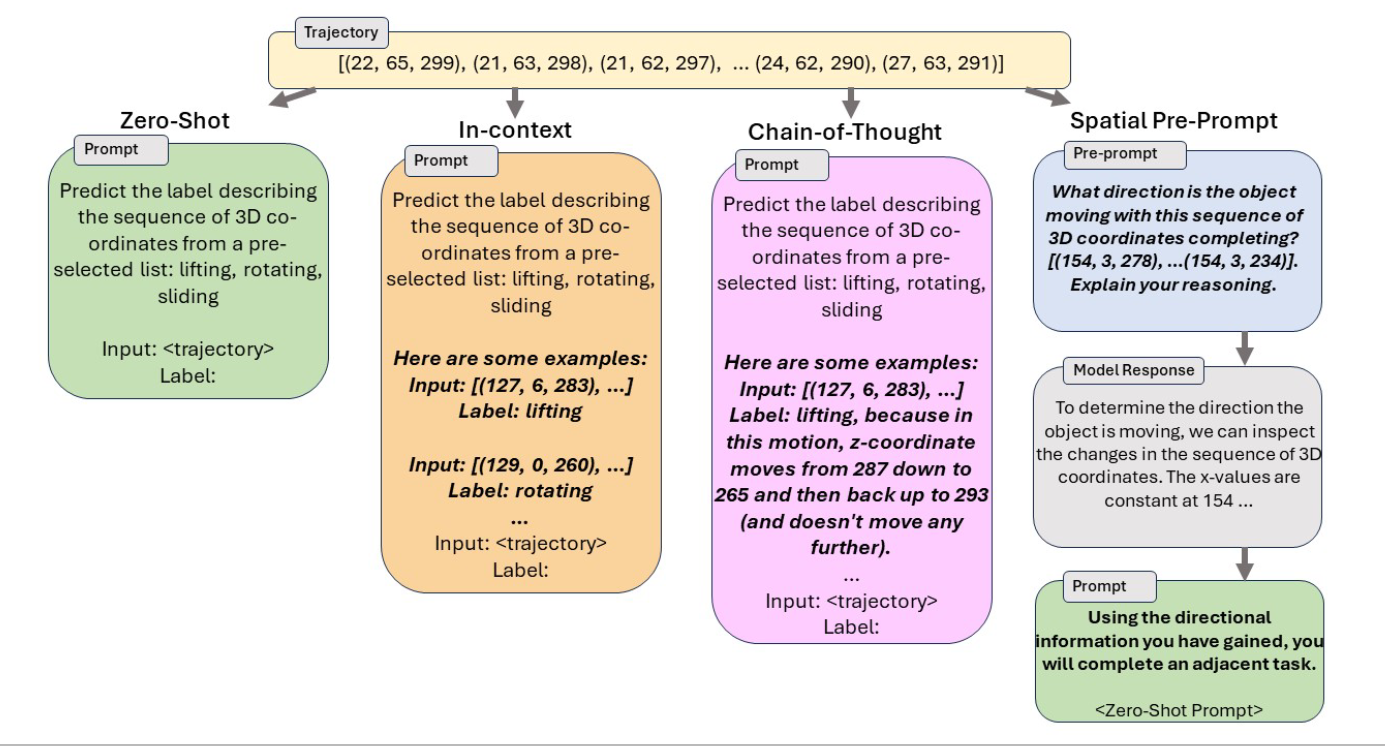
\includegraphics[width=0.9\textwidth]{Figs/SPP.png}
    \caption{Different Types of Prompting Mechanisms - Zero-shot, In-context Learning, Chain-ofThought and Spatial Prefix-Prompting.}
    \label{fig:spp}
\end{figure}

Another study \cite{sharma2023exploring} focused on improving the reasoning capabilities of LLMs like Llama, ChatGPT, etc., when processing 3D trajectory data of robots from the CALVIN dataset. The tasks involved include 2D directional and shaping labels. 
Unlike the datasets mentioned above, this dataset contains only the 3D coordinates of objects moving in space. Additionally, the researchers introduced a new method called prefix-based prompting, which improved the performance of LLMs by up to 33\% on the 3D trajectory dataset 
and by 10\% on the SpatialQA dataset using zero-shot prompting. The study found that while LLMs perform well on natural language reasoning tasks, they struggle with shape recognition and handling spatial relationships. Methods like in-context learning and chain-of-thought (CoT) prompting can enhance LLMs' reasoning capabilities; however, 
the authors’ Spatial Prefix-Prompting (SPP) method (\ref{fig:spp}) outperformed these approaches on most benchmarks. SPP works by using a set of simple, pre-prepared questions to encourage LLMs to answer and reason through straightforward problems first. The reasoning derived from these questions is then used to tackle more complex related questions
Not only does this method surpass CoT and few-shot learning in benchmarks, but it is also more efficient as it does not require explicit reasoning steps (as CoT does) and avoids bias introduced by provided examples (as in few-shot learning). 







\subsection{Causual Reasoning}
\input{Sections/methods/causual.tex}






\paragraph{Paragraphs}


There is also a \verb+\paragraph+ command available, which sets the heading in
bold, flush left, and inline with the text, with the heading followed by 1\,em
of space.




\section{Experiments and Results}
\subsection{Evaluating Casual Reasoning in Large Language Models}

\subsubsection{Introduction}
Based on the aforementioned methods for evaluating the causal reasoning abilities of large language models, in this section, we will conduct an assessment 
and examine the capabilities of modern language models in this type of reasoning through various prompting techniques.

\paragraph{Datasets} We evaluate using the COPA dataset, which is utilized for assessing causal reasoning abilities across a broad domain. 
COPA consists of 1000 questions, equally divided into two sets: a development set and a test set, each containing 500 questions (here, we will use the first 100 questions from the test set for evaluation). Each question includes a premise and two alternative choices. 
The primary task for LLMs is to provide answers A and B, such that the selected answer has a closer causal relationship to the premise.

\paragraph{Model and Prompting Techniques} To evaluate causal reasoning abilities, we conducted tests on four different models, all with a size of 7B parameters, including: Llama3-7B, Mistral-7B, Gemma-7B, and Qwen2-7B.
These are all newly released models that have achieved some impressive results in several LLM benchmarks. Simultaneously, we employed four different prompting methods: Few-shot learning + COT, Zero-shot learning + COT, Few-shot learning, and Zero-shot learning for each of the models mentioned above

\subsubsection{Results}
We performed inference using Ollama with the four models mentioned above, following the four different prompting approaches. Simultaneously, we used two metrics for evaluation: Accuracy and F1-score. This is appropriate because the task requires providing a correct result, specifically label A or label B. 
Below is a table comparing the results of each model across the different prompting methods (using 100 questions from the COPA dataset's test set).

\begin{table}[ht]
  \centering
  \begin{tabular}{|l|c|c|c|c|}
      \hline
      \textbf{Model}    & \textbf{Few-shot + COT} & \textbf{Few-shot} & \textbf{Zero-shot} & \textbf{Zero-shot + COT} \\ \hline

      Llama3-7B & 0.9, 0.87  & 0.88, 0.82  & 0.6, 0.62  & 0.73, 0.75  \\ \hline 

      Gemma2-7B & 0.94, 0.9 & 0.83, 0.86 & 0.7, 0.75 & 0.77, 0.8 \\ \hline 

      Mistral-7b & 0.95, 0.96 & 0.89, 0.91 & 0.62, 0.65 & 0.7, 0.72 \\ \hline

      Qwen2-7B & 0.97, 0.92 & 0.9, 0.86 & 0.72, 0.78 & 0.84, 0.84 \\ \hline

  \end{tabular}
  \caption{Comparison of models across different prompting methods (accuracy - left, F1-score - right)}
  \label{tab:model_comparison}
\end{table}


Based on the information provided in the table, it can be observed that most models achieve good results when using the few-shot learning method combined with COT. Conversely, using zero-shot alone does not yield high performance. 
This suggests that few-shot + CoT is an effective method for optimizing the causal reasoning ability of LLMs.Qwen2-7B demonstrates the best performance in most cases, particularly with the Few-shot + COT method (0.97). 
This indicates that it is a relatively strong model in terms of reasoning ability and well-suited for this type of prompting. Additionally, Gemma2-7B and Llama3-7B have relatively similar performance, with Gemma2-7B performing slightly better.

In summary, our experiment has yielded the following findings:

\begin{enumerate}
  \item The Few-shot + COT method is the most effective for enhancing causal reasoning abilities in LLMs.
  \item Qwen2-7B is the best-performing model in terms of causal reasoning, particularly with the Few-shot + COT method.
  \item Zero-shot learning alone is not effective for improving causal reasoning abilities.
\end{enumerate}


\section{Conclusion}
Please prepare submission files with paper size ``US Letter,'' and not, for
example, ``A4.''


Fonts were the main cause of problems in the past years. Your PDF file must only
contain Type 1 or Embedded TrueType fonts. Here are a few instructions to
achieve this.


\begin{itemize}


\item You should directly generate PDF files using \verb+pdflatex+.


\item You can check which fonts a PDF files uses.  In Acrobat Reader, select the
  menu Files$>$Document Properties$>$Fonts and select Show All Fonts. You can
  also use the program \verb+pdffonts+ which comes with \verb+xpdf+ and is
  available out-of-the-box on most Linux machines.


\item \verb+xfig+ "patterned" shapes are implemented with bitmap fonts.  Use
  "solid" shapes instead.


\item The \verb+\bbold+ package almost always uses bitmap fonts.  You should use
  the equivalent AMS Fonts:
\begin{verbatim}
   \usepackage{amsfonts}
\end{verbatim}
followed by, e.g., \verb+\mathbb{R}+, \verb+\mathbb{N}+, or \verb+\mathbb{C}+
for $\mathbb{R}$, $\mathbb{N}$ or $\mathbb{C}$.  You can also use the following
workaround for reals, natural and complex:
\begin{verbatim}
   \newcommand{\RR}{I\!\!R} %real numbers
   \newcommand{\Nat}{I\!\!N} %natural numbers
   \newcommand{\CC}{I\!\!\!\!C} %complex numbers
\end{verbatim}
Note that \verb+amsfonts+ is automatically loaded by the \verb+amssymb+ package.


\end{itemize}


If your file contains type 3 fonts or non embedded TrueType fonts, we will ask
you to fix it.


\subsection{Margins in \LaTeX{}}


Most of the margin problems come from figures positioned by hand using
\verb+\special+ or other commands. We suggest using the command
\verb+\includegraphics+ from the \verb+graphicx+ package. Always specify the
figure width as a multiple of the line width as in the example below:
\begin{verbatim}
   \usepackage[pdftex]{graphicx} ...
   \includegraphics[width=0.8\linewidth]{myfile.pdf}
\end{verbatim}
See Section 4.4 in the graphics bundle documentation
(\url{http://mirrors.ctan.org/macros/latex/required/graphics/grfguide.pdf})


A number of width problems arise when \LaTeX{} cannot properly hyphenate a
line. Please give LaTeX hyphenation hints using the \verb+\-+ command when
necessary.

\begin{ack}
Use unnumbered first level headings for the acknowledgments. All acknowledgments
go at the end of the paper before the list of references. Moreover, you are required to declare
funding (financial activities supporting the submitted work) and competing interests (related financial activities outside the submitted work).
More information about this disclosure can be found at: \url{https://neurips.cc/Conferences/2024/PaperInformation/FundingDisclosure}.


Do {\bf not} include this section in the anonymized submission, only in the final paper. You can use the \texttt{ack} environment provided in the style file to automatically hide this section in the anonymized submission.
\end{ack}

\section*{References}


References follow the acknowledgments in the camera-ready paper. Use unnumbered first-level heading for
the references. Any choice of citation style is acceptable as long as you are
consistent. It is permissible to reduce the font size to \verb+small+ (9 point)
when listing the references.
Note that the Reference section does not count towards the page limit.
\medskip


{
\small


[1] Alexander, J.A.\ \& Mozer, M.C.\ (1995) Template-based algorithms for
connectionist rule extraction. In G.\ Tesauro, D.S.\ Touretzky and T.K.\ Leen
(eds.), {\it Advances in Neural Information Processing Systems 7},
pp.\ 609--616. Cambridge, MA: MIT Press.


[2] Bower, J.M.\ \& Beeman, D.\ (1995) {\it The Book of GENESIS: Exploring
  Realistic Neural Models with the GEneral NEural SImulation System.}  New York:
TELOS/Springer--Verlag.


[3] Hasselmo, M.E., Schnell, E.\ \& Barkai, E.\ (1995) Dynamics of learning and
recall at excitatory recurrent synapses and cholinergic modulation in rat
hippocampal region CA3. {\it Journal of Neuroscience} {\bf 15}(7):5249-5262.
}





%%%%%%%%%%%%%%%%%%%%%%%%%%%%%%%%%%%%%%%%%%%%%%%%%%%%%%%%%%%%

\appendix

\section{Appendix / supplemental material}

\input{Sections/appendix.tex}

\bibliographystyle{plain}
\bibliography{mybib}

\end{document}